\begin{frame}{Temperatura} 
    \begin{itemize} 
        \item Associamos o conceito de temperatura a quão quente ou frio um corpo está quando nele
            tocamos, mas essa avaliação não é confiável nem quantitativa 
        \item Dizemos que dois ou mais corpos estão em \textbf{contato térmico} quando
            pode haver troca de \textbf{energia} entre eles devido à diferença de
            temperatura 
        \item Dizemos que dois ou mais corpos estão em
            \textbf{equilíbrio térmico} se quando forem colocados em contato térmico
            não houver troca de \textbf{energia} devido à diferença de temperatura, ou
            seja, estão na mesma temperatura 
            \begin{block}{Lei zero da Termodinâmica} 
                Se dois corpos estão em equilíbrio térmico com um terceiro,
                então os três corpos estão em equilíbrio térmico entre si 
            \end{block} \pause
        \item Assim, podemos pensar na temperatura como a propriedade que determina se
            um corpo está em equilíbrio térmico com outro 
    \end{itemize} 
\end{frame}
%
\begin{frame}
    \begin{itemize}
        \item Uma propriedade física que varia com a temperatura é chamada de
            \textbf{propriedade termométrica}
        \item Usando a lei zero e um corpo com uma propriedade termométrica
            mensurável, podemos construir um \textbf{termômetro}
        \item Colocamos o termômetro em contato térmico com um corpo A e
            medimos a propriedade termométrica no equilíbrio térmico
        \item Colocamos o termômetro em contato térmico com um corpo B e
            medimos a propriedade termométrica no equilíbrio térmico
        \item Se o valor medido para propriedade termométrica for igual para
            ambos os corpos, eles têm a mesma temperatura
        \item Além disso, podemos dar um valor para a temperatura a partir do
            valor medido da propriedade termométrica: podemos definir uma
            \textbf{escala termométrica}
    \end{itemize}
\end{frame}
%
\begin{frame}
    \frametitle{Algumas escalas}
    \begin{itemize}
        \item A \textbf{escala de temperatura centigrada ou Celsius} define a
            temperatura do ponto de gelo como sendo \SI{0}{\celsius} e a
            temperatura do ponto de vapor como sendo \SI{100}{\celsius}
        \item A \textbf{escala de temperatura Fahrenheit} define a temperatura
            do ponto de gelo como sendo \SI{32}{\degree F} e a temperatura do
            ponto de vapor como sendo \SI{212}{\degree F}
        \item Existe uma temperatura na qual um termômetro em Celsius e um em
            Fahrenheit marquem o mesmo valor? Qual é essa temperatura?
    \end{itemize}
\end{frame}

\begin{frame}

    \frametitle{Algumas questões...}
    \begin{enumerate}
        \item Ao se calibrar um termômetro que apresentava defeito,
            verificou-se que ele indicava \SI{2}{\degree} para a temperatura do
            ponto de gelo e \SI{98}{\degree} para o ponto de ebulição da água.
            Qual seria a temperatura Celsius correta quando o termômetro
            indicasse \SI{-10}{\degree}? 

        \item Em uma escala hipotética X, foi associado à temperatura de fusão
            do gelo o valor de \SI{-20}{\degree X} e à temperatura de ebulição
            da água o valor de \SI{580}{\degree X}. Obtenha a expressão
            matemática que relaciona uma temperatura qualquer, \(T_X\), com a
            temperatura correspondente, \(T_C\), na escala Celsius.
    \end{enumerate}
\end{frame}

\begin{frame}
    \frametitle{A escala de temperatura absoluta ou  escala Kelvin}

    \begin{itemize}
        \item Um gás ideal é definido como um gás onde a pressão, o volume e a temperatura se relacionam pela expressão
            \[
                PV=nR(T-T_0)
            \]
            onde R=\SI{8.314}{J/(mol\ K)}, \(n\) é o número de moles do gás e \(T_0\) é a temperatura onde \(P=0\)

        \item A característica principal da escala de temperatura absoluta ou
            Kelvin é o zero: na temperatura de \SI{0}{K} temos $P=0$

        \item Só falta definir outra temperatura para termos uma escala: a
            temperatura do \textbf{ponto triplo} da água (\SI{273.16}{K})

        \item \(T_0 = \SI{-273.15}{\celsius}\) e o ponto triplo da água ocorre
            em \(T=\SI{0.01}{\celsius}\) sob uma pressão de \SI{4.58}{mmHg}

    \end{itemize}
\end{frame}


\begin{frame}
    \frametitle{Calor e energia interna}
    \begin{itemize}
        \item \textbf{Energia interna} é toda a energia de um sistema associada a seus
            componentes microscópicos -- átomos e moléculas -- \textit{quando vistos em
                um sistema de referência em repouso com relação ao centro de massa do
            sistema}. Essa última parte exclui a energia associada a fatores externos ao
            sistema, por exemplo, a energia cinética devido a movimentação pelo espaço

        \item \textbf{Calor} é definido como a transferência de energia através do
            limite de um sistema \textit{devido a uma diferença de temperatura} entre o
            sistema e sua vizinhança

            \begin{itemize}
                \item Calor \textbf{não é} a energia em uma substância quente
                \item Calor \textbf{não é} radiação emitida por uma substância quente
                \item Calor \textbf{não é} a ''quentura'' de uma substância
            \end{itemize}
    \end{itemize}
\end{frame}

\begin{frame}

    A unidade de medida SI do calor é a mesma da energia, o joule.
    \begin{itemize}
        \item A caloria (cal) é definida como a quantidade de energia transferida
            necessária para elevar a temperatura de \SI{1}{g} de água de
            \SI{14.5}{\celsius} para \SI{15,5}{\celsius}
            \[
                \SI{1}{cal} = \SI{4,186}{J}
            \]

        \item A unidade térmica britânica (Btu) é definida como a quantidade de energia
            transferida necessária para elevar a temperatura de \SI{1}{libra}
            (\SI{4,448}{N}) de água de \SI{63}{\degree F} para \SI{64}{\degree F}
            \[
                \SI{1}{Btu} = \SI{252}{cal} = \SI{1054}{J}
            \]
    \end{itemize} 
\end{frame}

\begin{frame}
    \frametitle{Capacidade térmica e calor específico}
    A quantidade de energia Q necessária para aumentar em \SI{1}{\celsius} a
    temperatura de uma \textbf{amostra} de uma substância é chamada de capacidade
    térmica da amostra
    \[
        C=\frac{Q}{\Delta T}
    \]

    O calor específico de uma substância é dada por
    \[
        c=\frac{C}{m}
    \]

    onde $m$ é a massa de uma amostra da substância que possui capacidade térmica $C$
\end{frame}

\begin{frame}
    \frametitle{Calor latente}

    \begin{itemize}
        \item Durante uma \textbf{mudança de fase} a temperatura permanece constante. A
            energia absorvida ou liberada é usada na transformação

        \item Para uma substância pura, a mudança de fase a uma dada pressão ocorre
            apenas em uma temperatura específica

        \item A energia necessária para congelar uma amostra de uma substância de massa
            $m$ é proporcional à massa da amostra
            \[
                Q_s= -mL_s
            \]
            onde $L_s$ é o calor latente de solidificação da substância

        \item Se a mudança de fase é de líquido para gás. temos
            \[
                Q_v = +mL_v
            \]
            onde $L_v$ é o calor latente de vaporização
    \end{itemize}
\end{frame}

\begin{frame}
    \frametitle{Trabalho na Termodinâmica}
    \begin{itemize}
        \item Podemos aumentar a temperatura de um sistema realizando trabalho sobre ele
        \item Na figura abaixo está um diagrama do aparato que Joule usou para
            determinar o trabalho necessário para aumentar a temperatura de uma quilo
            de água em \SI{1}{\degree C}
    \end{itemize}
    \begin{center}
        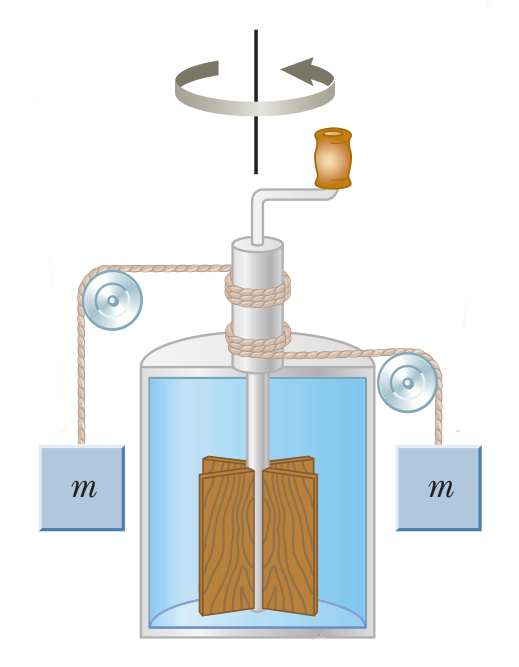
\includegraphics[width=0.25\textwidth]{images/joule.png}
    \end{center}
\end{frame}

\begin{frame}[c]
    \begin{itemize}
        \item Através desse experimento Joule descobriu que era necessário
            \SI{4,184}{kJ} para aumentar a temperatura de \SI{1}{kg} de água em
            \SI{1}{\degree C}, ou seja
            \[
                \SI{1}{cal} = \SI{4,184}{J}
            \]

    \end{itemize}
\end{frame}

\begin{frame}
    \frametitle{Trabalho realizado sobre um gás ideal por uma pressão constante}
    Seja um gás ideal confinado em um cilindro com um pistão bem ajustado e sem atrito
    \begin{center}
        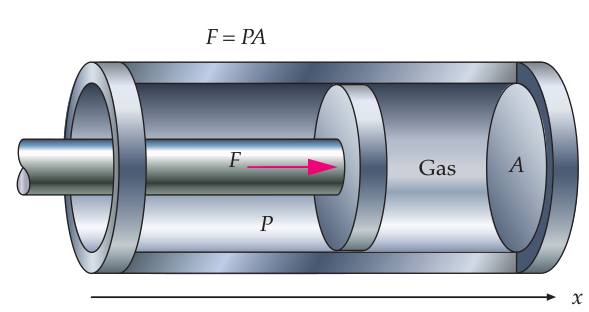
\includegraphics[width=0.425\textwidth]{images/quasistatic}
    \end{center}
    \begin{itemize}
        \item Quando o pistão se move uma pequena distância $\Delta x$, o trabalho realizado \textit{sobre o gás pelo pistão} é
            \[
                W_{\text{sobre~o~gás}} = F_x \Delta x=PA \Delta x=-P\Delta V
            \]
        \item Observe que para uma compressão $\Delta x > 0$ mas $\Delta V < 0$, enquanto que para uma expansão ocorre o contrário
    \end{itemize}

\end{frame}
